\section{Background and Model}
\label{sec:model}

\begin{figure*}[t]
\begin{center}
\includegraphics[scale=0.5]{figures/cloudflow2.eps}
%\vspace{30pt}
\caption{\small 
% 
Administrators from different departments provide CloudFlow with VM images
and desired security policies.  CloudFlow (CF) deploys the images to the
cloud and propagates CF policies automatically to relevant nodes.  The
policies are then used to dynamically deduce CF labels for VMs.  Policies
are enforced in real-time using VM introspection and call-backs to the management module(e.g. 
migration requests).  The figure shows a migration in progress.
%
\label{cloudflow:figure:highlevelarch}}
\end{center}
\end{figure*}


\paragraph{\bf Regulatory compliance \& Information flow control}
%What are they
%Regulatory compliance and information flow control
%make 1 paragraph out of both of the two belows - > all these things require information flow control

%People do not trust institutions when they believe that the appropriate policies to deter abuse are lacking or not being enforced. When the public trust is threatened, often new regulations and policies are put into place to restore trust. For example, Enron was a leading energy company in the 1990s that went bankrupt in 2001 \cite{Enron}. Enron's pensioners, employees, and ordinary shareholders suffered huge financial losses while Enron's top management made hundreds of millions of dollars from selling stock at prices inflated by fraudulent financial reporting. Instead of stopping the fraud, Enron's accounting auditor, Arthur Andersen, helped carry it out, then tried to destroy the evidence \cite{AP02}. To restore public trust in the financial accountability of publicly-traded corporations, Congress passed the Sarbanes-Oxley Act \cite{Sox} in 2002. To comply with SOX, companies have had to make fairly expensive changes to their IT processes; Congress's intent is that the cost of these changes is much less than the cost to society of not being able to trust corporate financial reports. Similarly, compliance with the Health Insurance Portability and Accountability Act \cite{HIPAA} has been quite expensive, but presumably much less than the societal cost of errors, omissions, and inappropriate disclosure of medical records.

%HIPAA and SOX created markets for new IT products that could increase assurances at reasonable cost. As society increases its reliance on electronic delivery of services from government, business, and educational institutions, new trust issues will continue to arise, and trust-related legislation and opportunities for new technology that increases trust will continue to grow. Already there are many major regulations that address IT trust issues, including the Gramm-Leach-Bliley Act \cite{GLB}, Federal Information Security Management Act \cite{FISMA}, Securities and Exchange Commission (SEC) rule 17a-4 \cite{SEC17cfr241}, Food and Drug Administration 21 CFR Part 11 \cite{FDA21cfr11}, the Family Educational Rights and Privacy Act \cite{FERPA}, the e-Government Act \cite{EGA}, and the Patriot Act \cite{Pat01}.

People do not trust institutions when they believe that the appropriate
policies to deter abuse are lacking or not being enforced.  When the public
trust is threatened \cite{Enron}, often new regulations and policies are put
into place to restore trust.  Over 10,000 IT-impacting regulations exist in
the US alone, including Sarbanes-Oxley Act \cite{Sox}, Health Insurance
Portability and Accountability Act \cite{HIPAA}, Gramm-Leach-Bliley Act
\cite{GLB}, Federal Information Security Management Act \cite{FISMA},
Securities and Exchange Commission (SEC) rule 17a-4 \cite{SEC17cfr241}, the
e-Government Act \cite{EGA}, and the Patriot Act \cite{Pat01}.

%strongly link all of the above to information flow control

The core issue that many of these laws ultimately address is the need for
fair and transparent control of sensitive information.  Accordingly,
information flow control is an essential necessity within any large
organization.  However, with scale come increasing difficulties in enforcing 
information flow control, and illicit accesses can go unmonitored.

%too  many often
\paragraph{\bf MLS and Chinese Wall policies}
%
Of particular importance in regulatory contexts are Chinese Wall policies
that institutions need to enforce to mitigate existing and potential
conflicts of interest.  A \textit{Chinese Wall} is a barrier placed
across information flow within an organization that aims to segregate
employees who have access to sensitive information from those who may
use this information for personal gain.  Traditionally this is
done by isolating personnel from each other and monitoring information
access and sharing.  As we will see, CloudFlow can naturally enforce Chinese
wall policies by dynamic inter-VM segregation for applications running on
behalf of principals under regulatory constraints.

% MLS systems process information with differing, often incompatible,
% security levels.  They provide access control mechanisms for users at
% different security clearances and needs-to-know, and thus prevent
% illegitimate access to information.

Similarly, in intelligence and defense scenarios, information flow control
is subject to \textit{Multilevel security} (MLS) policies.  MLS systems
process information that exists at differing, often incompatible, security
or \textit{classification levels} and provide access control mechanisms for
users at different security clearances and needs-to-know, preventing
illegitimate access to classified information.  One popular example 
is the well known Bell-Lapadula confidentiality policy model
\cite{BellLapadula}.  Traditionally, Bell-Lapadula uses four different
classification levels, from Top Secret down to Unclassified. Information
flow is controlled according to ``no reads up, no writes down'' rules. 
% incorrect:
% Other MLS models, such as the Biba model \cite{Biba}, exist
% for enforcing data integrity instead of confidentiality.  
CloudFlow can also naturally enforce MLS policies as will be shown later.

There has been previous work on network-centric cloud-wide policy
enforcement \cite{CloudEncPolicy10,NetODESSA,CloudProfit12,CloudPower12,AllocationPolicy10}. Policies are usually defined in order to attain better
segregation amongst nodes of different computational and storage needs and
provide better load balancing or scheduling algorithms.  Work that most
closely resembles CloudFlow includes a result that proposes stronger VM isolation
mechanisms \cite{Mushi}.  Such mechanisms rely mainly on providing
rudimentary MLS via hardwired network isolation.


\paragraph{\bf Side Channels}
%Side channels exist wherever you have information leakage

\begin{wrapfigure}{L}{0.16\textwidth}
\vspace{-10pt}
\includegraphics[width=0.20\textwidth]{figures/memh2.eps}
\vspace{-25pt}
\label{cloudflow:figure:memh}
\end{wrapfigure}

% An organization that has information flow control procedures in place may
% still be susceptible to information leakage via \textit{side channel
% attacks}.  
In a {\em side channel attack} information is gained
from a system using a resource that is shared between an unsuspecting victim and a perpetrator.  Examples of such shared resources include power conduits, discs, shared memory hierarchies etc. all of which can be used to infer potentially sensitive information illegitimately.

An especially important and interesting class of side channels arises due to
improper VM isolation.  This derives from the inherent resource sharing
design that comes with efficient infrastructures.  For example, clouds
usually multiplex multiple VMs on the same underlying hardware by assigning
a virtual CPU (VCPU) to each VM.  The number of VCPUs can be greater than
the physical CPUs and hence, in the case of load balancing a large number of
VMs, different VCPUs end up getting mapped to the same physical CPU.  Two
VMs on the same physical CPU end up sharing all levels of the memory
hierarchy.  This can lead to information leakage e.g.,  via shared caches
\cite{SideCloud,SideCrypto}.  Even though the two VMs share no explicit
state, the CPU cache is a shared resource impacted by the internal state of
both VMs (see Figure).  This
introduces a side channel that potentially breaks desired information flow
control invariants.  Numerous other side channels have been discovered in a
variety of settings and have been studied extensively
\cite{SideCloud,SideCrypto,LastSummer,ScriptlessAttacks}.  Associated
exploits have been designed and implemented to extract private information
such as RSA and AES keys \cite{SideCloud,SideCrypto,PrimeProbe12} via side channels from
unsuspecting victims.

While preventing individual side channels at OS and hypervisor level is
difficult and arguably impossible to achieve in efficient resource sharing
systems, we believe a unique mitigation opportunity exists at cloud level. 
By reactively enforcing information flow control invariants through runtime
introspection and on-demand VM migration the effects of existing side channels can be mitigated.
However we acknowledge the fact that any system that is reactive in nature can be subject to 
{\em residual side channels} i.e. whenever a policy is enforced at runtime the attacker has the opportunity 
to learn information about the policy being enforced. This is not an issue in the regulatory compliance scenario 
under focus in this paper as policies themselves are not classified information and do not need to be protected from side channel attacks.
% Thus our technique is preventive in nature.

\paragraph{\bf VM Introspection}

Introspection was
first suggested in the seminal work of Garfield and Rosenblum \cite{Terra}. 
Two types of introspection mechanisms exist: those requiring changes to the
guest VM or target applications, and those that work externally at the hypervisor level.  CloudFlow aims for maximum
transparency and minimizing the impact on guest OSes and applications and
thus uses external introspection.

Introspection has been extremely popular in the recent past
\cite{RemoteAttestation,OutOfBox,OutOfBoxMalware,AntFarm,VMIObserve,TamperResist,libvmi}. 
Previous introspection mechanisms have been aimed towards solving problems such as intrusion detection \cite{CoPilot}, malware analysis
\cite{Ether} and forensics.  

External introspection approaches however are inherently at a disadvantage
due to having an outsider view and remain prone to the {\em semantic gap}
problem \cite{chen01virtual,SemanticGap}, the difficulty of mapping between
low-level hardware events and higher-level system abstractions.  Further, in
practice, interpreting the memory of a running guest OS can be error prone,
and subject to attacks \cite{DKSM}.

In recent years there has been much effort to reduce this gap and gain
meaningful, detailed information even in the case of non-cooperating,
adversarial guest VMs \cite{Virtuoso,ProcessImplanting}.  This has led to
the construction of hybrid approaches that install an agent inside the monitored
guest as well, to provide a view that is richer in semantics.

%Why are they used
\paragraph{\bf Clouds}
% 
Cloud computing enables the outsourcing of computation and storage needs to
an infrastructure managed by a third party (public cloud provider, or
in-house company-wide cloud/IT department).  Clouds today are mostly
virtualization based i.e.  they use VMs as the basic unit for leasing out
computation.  They usually provide a management front-end which can be used
as an input point to deploy and manage workload-personalized VMs which are
run in a data center composed of physical nodes that provide
computation and storage, and can host multiple VMs simultaneously.  

CloudFlow is based on the OpenStack \cite{OpenStack} framework. OpenStack
offers a variety of services including computing and storage nodes, and
works with a wide range of hypervisors.  OpenStack is research friendly and
provides open source code which facilitated our design.  In addition, we
have picked the popular KVM-QEMU as our hypervisor of choice. Nevertheless we note that CloudFlow is hypervisor agnostic and it can be easily ported to other cloud platforms.

%Insert deployment model here
%who are users. how are labels acquired. what is deployed. what are labels. ideally we want to be able to write policy based on any guest state. however cloudflow currently only looks at labels. why?

\paragraph{\bf Deployment Model}
% 
The key idea behind CloudFlow is to enable hypervisors and the cloud
management layers to dynamically enforce cloud-wide information flow
policies that are based on guest VM state introspected at runtime.  For
example, in the case of Bell-Lapadula/MLS enforcement, a policy may specify
that no VM running applications classified/labeled as "confidential" can be hosted
on the same physical node as a VM running an application handling "top
secret" labeled data. No application and guest OS changes should be required. 

Naturally, the granularity at which guest state can be monitored via
introspection can vary vastly depending on the depth of data extracted from
the monitored kernel.  For illustration purposes, the current version of
CloudFlow allows policies containing references to SELinux labels of
guest-hosted processes.  The set of labels is currently derived from the
typing system put in place by SELinux inside each guest.

\paragraph{\bf Threat Model \& Assumptions}
% 
Of major concern are insiders who will benefit from cross-VM side channels.
Our main insight is that while at individual node level, the prevention
of side channels is tantamount to sacrificing efficiency, at cloud level we
can reactively prevent undesired side channels by intelligent on-demand
policy-enforcing VM placement, without a significant performance hit.

We trust the hypervisor, cloud administrators and policy designers. All
other users are untrustworthy.

Typically attackers will deploy a a malicious VM through which they will
attempt to exploit a known hardware side channel and extract sensitive
information from a unsuspecting target VM.  We assume that the adversary is
not in control of the entire underlying hardware and is unable to
bypass the hypervisor isolation.

Further, while we do not fully trust the guest OS and its applications, we
assume that guest kernels do not aim to subvert the introspection mechanism. 

Nevertheless, we note that recent work \cite{DKSM} has shown it is possible to deceive hypervisor
based introspection mechanisms via an attack on the guest kernel. This is
why ideally the guest OS should be entirely untrusted.

For this reason we designed a framework that can be ultimately independent
of guest support.  Additionally, we note that because CloudFlow does not modify the guest OS it does not need constant maintenance upon every kernel version update. CloudFlow can run on multiple kernel versions and different operating systems by simply changing how the introspection is performed externally. Finally, CloudFlow allows us to set a base for the policy
management and information flow control that remains agnostic of how the
guest state is actually acquired.

In ongoing work we are developing deception-robust introspection mechanisms that can
handle fully malicious guest kernels.

\begin{figure}[t]
\begin{center}
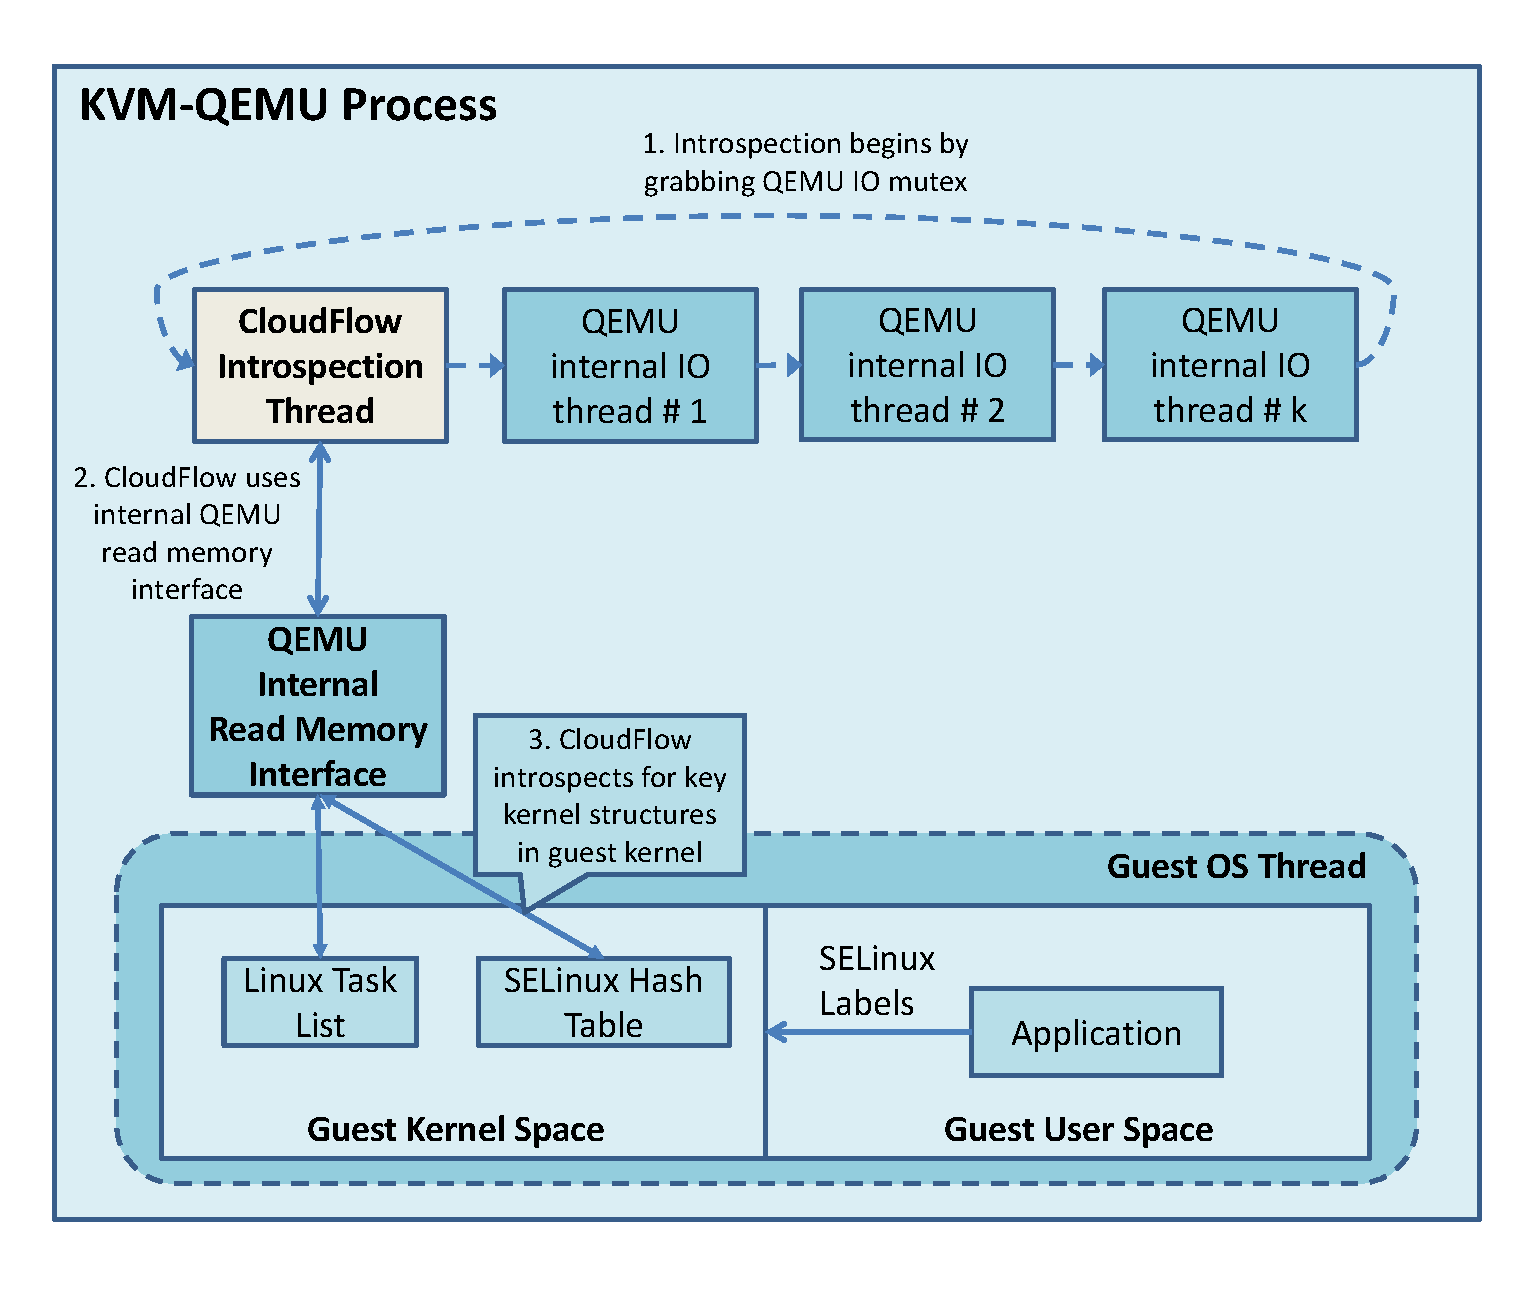
\includegraphics[scale=0.3]{figures/introspectionmodule2.eps}
%\vspace{30pt}
\caption{\small 
%
CloudFlow deploys a fast introspection thread that uses KVM-QEMU internals
directly to extract key kernel structures and infer information about tasks
running inside the guest OS.
%
\label{clowdflow:figure:introspectionmodule}}
\end{center}
\end{figure}

